\chapter{Experimental Methods} \label{cha:2}
%\lipsum[77]

\section{Materials}
%\lipsum[78]
All reactives were purchased from commercial suppliers. %and non further chemical modification or purification was done unless stated before.

\begin{itemize}
\item Chromium etchant: Standard, Sigma Aldrich
\item Gold etchant: Standard, Sigma Aldrich HHPAA (2-Hydroxy-4’-(2-hydroxyethoxy)-2-methylpropiophenone), 98$\%$, Sigma Aldrich 
\item Developer: AZ 726 MIF Developer, Merck performance Materials GmbH
\item EG: Ethylene glycol, $\geq$ 95$\%$, Sigma Aldrich
\item $[$EMIM$][$EtSO$_{4}]$: (1-Ethyl-3-methylimidazolium ethyl sulfate), $\geq$95$\%$, Sigma Aldrich 
\item MBBAm: (N,N’-Methylenebisacrylamide), 99$\%$, Sigma Aldrich 
\item NIPAm: (N-Isopropylacrylamide), 97$\%$, Alfa Aesar 
\item Sacrificial Layer 1: Sacrifical Layer 1 (SL1), Orthogonal Inc
\item Photoresist: AZ 1518 Photoresist, Merck Performance Materials GmbH \& Microchemical GmbH
\item Photoresist for undoped species: NLOF 2020, commercial negative-tone photoresist, Microchemical
\item Orthogonal Photoresist for doped species: OSCoR 4020 Photoresist, Orthogonal Inc.
\item Developer for SL1: Developer HF 7300, Orthogonal Inc.
\item Orthogonal Developer for OSCor 4020: Orthogonal Developer 103a, Orthogonal Inc.
\item Orthogonal Stripper: Orthogonal Stripper 900, Orthogonal Inc. 
\item p(g3T2-T): 3-(2-(2-(2-methoxyethoxy)ethoxy)ethoxy)thiophene
\item Dopants: 1,3,4,5,7,8-hexafluorotetracyanonaphthoquinodimethane (F$_{6}$TCNNQ) and 1,3,4,5-tetrafluorotetracyanonaphthoquinodimethane (F$_{4}$TCNQ)
\item Adhesion promoter: Silane A174 (3-(Trimethoxysilyl)propyl methacrylate), TCI

\end{itemize}

\section{Equipment}
\begin{itemize}
\item Baking: All baking steps were carried out on a Stuart SD160 digital hotplate (Stuart Equipment, UK). 
\item Electrical characterization (ambient): Device characterization under ambient conditions was performed on a Everbeing C-6 Probe Station (Everbeing Int’l Corp., Taiwan), connected to a Keithley 4200-SCS Semiconductor Characterisation System (Keithley Instruments, USA). 
\item Electrical characterization (glovebox): Device characterisation was performed in a nitrogen-filled glovebox. Probing needles were connected to two Keithley 236 Source Measure Units (Keithley Instruments, USA). 
\item Cyclic voltammetry and Impedance measurements: Measurements were carried out by using a Metrohm Autolab PGSTAT302N potentiostat/galvanostat (Metrohm AG, Switzerland).
\item Micrographs: Micrographs were taken on a Nikon Eclipse LV100ND microscope, equipped with a DS-Fi2 camera (Nikon, Japan). 
\item Photolithography: Photolithography was carried out on a SÜSS Microtec MJB4 maskaligner system (SÜSS Microtec AG, Germany). 
\item Photomasks: Photomasks were custom made by Compugraphics Jena in a 4-inch format (soda-lime glass covered with chromium) and held several mask designs (Compugraphics Jena GmbH, Germany). 
\item Plasma cleaning: O$_{2}$-plasma cleaning was performed by using a Harrick PDC-002 plasma cleaner (Harrick Plasma, USA), connected to a Leybold Heraeus Combitron CM 330 Vacuum Gauge Controller (Leybold GmbH, Germany). 
\item Plasma etching: O$_{2}$-plasma etching was performed by using a Diener electronic ATTO plasma cleaner (Diener electronic GmbH \& Co. KG, Germany). 
\item Profilometry: Profilometry was performed on a Veeco Dektak 150 surface profiler (Veeco Instruments Inc., USA).
\item Film resistance measurements: The film resistance was measured using a linear four-point probe system (Lucas four-point probe connector) connected to a multimeter (Keithley 2010 Multimeter).
\item Transmittance and Reflectance measurements: Measurements were performed with UV-Visible-NearInfraRed Spectroscopy on a SolidSpec-3700 UV-Vis-NIR spectrometer using an integral sphere from Shimadzu.
\item Energy of HOMO/HBEC cutoff measurements: Measurements were done using Ultraviolet Photoelectron Spectroscopy (UPS) on a PHOIBOS 100 from Specs, a Helium plasma discharge lamp (UVS10/35, Specs).
\item Spincoating: Samples were coated with a SAWATEC SM-180-BT spincoater (SAWATEC AG, Switzerland).
\end{itemize}

\section{Software} \label{param}
%% Add citations of libraries and stuff
\begin{itemize}
\item Data processing: All data was processed by customized scripts written in Python. Files import and manipulation was done by using OS \cite{os_module} and CSV \cite{csv_module} modules. Mathematical computations (e.g. fits, integration) were carried out by employing the NumPy \cite{numpy_2012}, SciPy \cite{scipy_linreg}, and PeakDetect \cite{peakdetect} libraries. Visualisations were performed using the Matplotlib library \cite{matplotlib_2012}. All is compiled in the following GitHub Repository: \href{https://github.com/marivelascoe25/Thesis.git}{\textbf{marivelasco25/Thesis.git}}.
\item Electrical characterisation: Measurements were performed by controlling SMUs through the in-house developed SweepMe! software \href{https://sweep-me.net/}{\textbf{(https://sweep-me.net/)}}. 
\item Profilometry: Profilometry was performed by using the Dektak software (Veeco Instruments Inc., USA).
\item Cyclic voltammetry: Measurements were performed by using the NOVA software (Metrohm AG, Switzerland). Parameters were fixed and are described in the following table: 

\begin{table}[h]
	\centering
	\caption{Cyclic Voltammetry parameters.}
	\begin{tabular}{r r} \hline
		Parameter	& Value \\ \hline
		Start/Stop potential	& 0 V \\ 
		Upper vertex potential	& 1 V \\ 
		Lower vertex potential	& -1 V \\ 
		Number of scans	& 10 \\ 
		Scan rate	& 0.1 V/s \\ \hline
		%Step	& 0.05 \\ 
	\end{tabular}
	\label{tab:CV}
\end{table}

\item Impedance measurements: Measurements were performed by using the NOVA software (Metrohm AG, Switzerland) in potentiostatic mode. Parameters were fixed and are described in the following table: 

\begin{table}[h]
	\centering
	\caption{Electrochemical Impedance Spectroscopy parameters.}
	\begin{tabular}{r r} \hline
		Parameter	& Value \\ \hline
		Initial frequency	& 10$^{5}$ Hz  \\ 
		Final frequency	& 10$^{-1}$ Hz \\ 
		Frequencies per decade	& 10 \\ 
		Amplitude (V$_{RMS}$)	& 0.01 V \\ \hline
	\end{tabular}
	\label{tab:EIS}
\end{table}

%105 - 10-1
%10 frequencies per decade
%Amplitude 0.01 VRMS

\end{itemize}

%\section{Photomasks}
%Photomasks were employed during photolithography to cover or uncover the respective areas of interest, depending on the photoresist employed (positive or negative, respectively). Details are given in Chapter . The employed photomasks for OECT fabrication are shown in Figure , with a labeled close-up scheme of a transistor device given in Figure . All devices were designed in a side-gate structure with the 16 devices each mask comprised differing in channel length and gate distance. An overview of the specific dimensions is provided in Table  with the designations assigning the devices (U1 – U8 (Up) and D1 – D8 (Down)). Since investigations on device dimensions were not a direct study object of this work, according assignments were left out. However, all comparisons between different substrates do of course always refer to the very same devices on each individual sample. A device assignment of all plots shown is given in Table S1. It shall be pointed out that the fabrication process did regularly lead to samples with several non-functioning devices. Accordingly, experiments were to be conducted on OECTs that were found working, which accounts for the variation in examined devices. For experiments of Chapter , available photomasks were arranged and covered to yield the setup shown in Figure . For experiments of Chapter , channels of p(g3T2-T) with underlying gold contacts were prepared. The corresponding photomasks are shown in Figure  and were printed on plastic foil in a common inkjet printer. As schematically shown in Figure  though, the lower big as well as several small gold contacts have not been used during execution. The lowest small gold contact served as source electrode.

\section{Experimental Procedures}

All fabrication steps were performed under standard cleanroom conditions.
\subsection{Preparation of Films} \label{subsec:films}
\paragraph{Dynamic spin-coating of p(g3T2-T).}Unlike reference \cite{tanTuningOrganicElectrochemical2022}, in which drop cast is used to deposit undoped and doped p(g3T2-T), in order to perform photolithography and being able to do a miniaturization process, homogeneous films are needed. Dynamic spin-coating was previously stablished by BioSens group members at IAPP, due to the high volatility of p(g3T2-T) solvant: chloroform. Substrates were cleaned using subsequent steps of ultrasonic bath with acetone for 15 minutes, IPA rinsing, N$_{2}$-drying and O$_{2}$-plasma etching for 5 min (0.3 mbar). Then, 70$\mu$L of 10 mg/mL of p(g3T2-T) mixed at 60$^{\circ}$C for 20 minutes, was dynamic-spin-coated at 3000 RPM for 60s, to yield approximately 70nm-thick films. Dry sample at 80$^{\circ}$C.

\paragraph{Dynamic spin-coating of F$_{4}$TCNQ dopant.}Different doping levels of p(g3T2-T) were achieved by dynamic spin-coating 140$\mu$L of dopants at different concentrations (5, 10 and 20 mg/mL), previously mixed in acetronitrile at $60^{\circ}$C for 20 minutes. Dry sample at 80$^{\circ}$C.

\begin{figure}[ht]
  \centering
  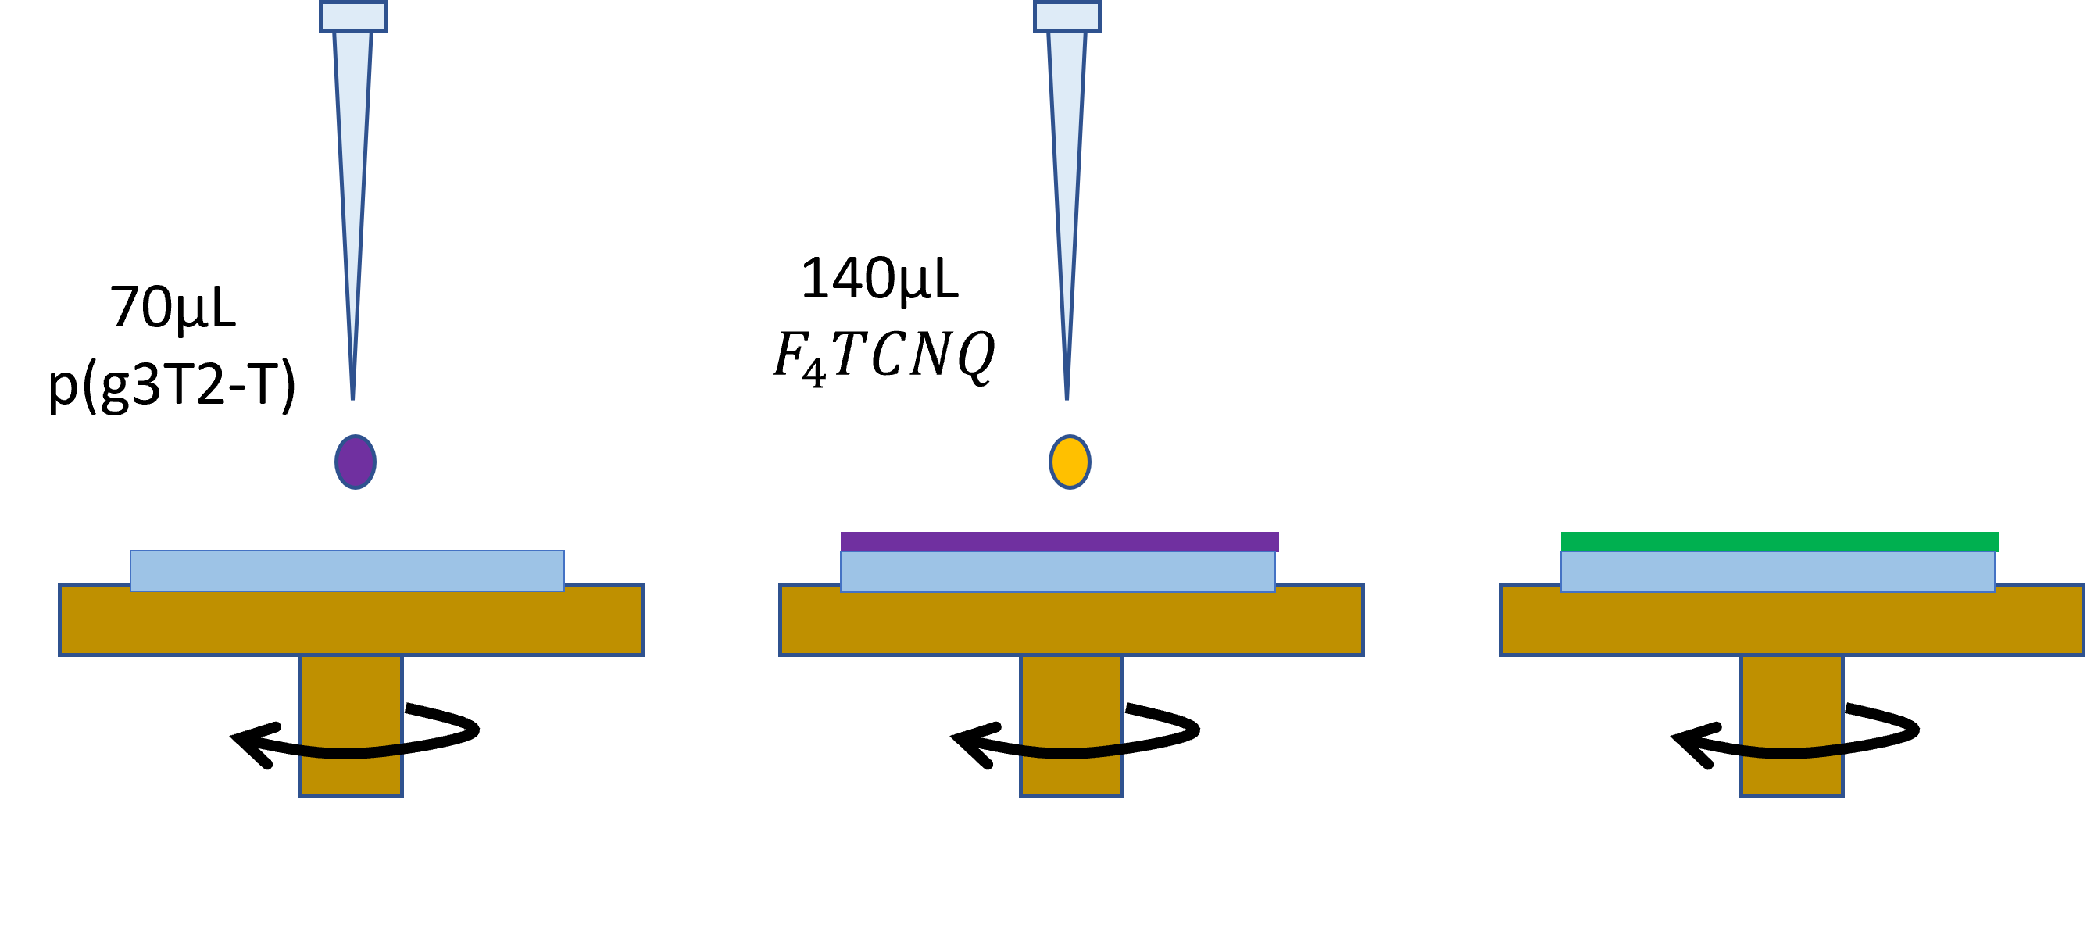
\includegraphics[width=10cm]{Images/pdf/spin_coating.pdf}
  \caption{Dynamic spin-coating process to obtain undoped and doped films of p(g3T2-T)).}
  \label{fig:coating}
\end{figure}

\subsection{Doping Characterization of Films}

\paragraph{UV-Vis-NIR Spectroscopy.}After the preparation of the films, transmittance (T) and reflectance (R) was measured using the UV-Vis-NIR Spectrometer in the range of 285 to 1600 nm, and slit width of 5.0 nm. Then absorption (A) was calculated via


\begin{equation}\label{eq:abs}
	A = 1 - T - R,
\end{equation}

and normalized with respect to the incoming light \cite{uvvis}. Additional measurements were taken, after some days of storage under ambient conditions to check its stability on air.

\paragraph{Ultraviolet Photoelectron Spectroscopy.}After the preparation of the films, %(air exposure) 
the energy of the highest occupied molecular orbital cutoff (E$_{HOMO}$) and the high binding energy cutoff E$_{HBEC}$ was measuring using UPS. The pressure in the chamber during measurements was about 5$\cdot$10$^{-9}$ mbar, while the base pressure is in the range of 10$\cdot$10$^{-10}$ mbar. The workfunction (WF) and ionization energy (IE) are calculated by using the following equations:

\begin{equation}\label{eq:wf}
	WF = h\nu - E_{HBEC} \quad [eV],
\end{equation}

\begin{equation}\label{eq:ie}
	IE = h\nu - (E_{HBEC}-E_{HOMO}) \quad [eV],
\end{equation}

where $h\nu = 21.22 eV$, the main He I excitation line of the Helium plasma discharge lamp \cite{buchholtzDopingPropertiesNovel2021}. 

\paragraph{Profilometer.}The films were scratched 4 times to remove part of material, and measure the cavity depth to obtain the film thickness.

\paragraph{Four-point probe.}Sheet resistance was calculated via

\begin{equation}\label{eq:rs}
	R_{S} = \frac{\pi}{ln(2)}R = 4,53 R \quad [\Omega/sq],
\end{equation}

where R is the resistance measured with the four-point probe setup and resistivity was calculated using the following equation:

\begin{equation}\label{eq:resist}
	\rho = R_{s}t \quad [\Omega.cm],
\end{equation}
 
%\subsection{Roughness characterization of films} 

\subsection{Fabrication of Organic Electrochemical Transistors}

\subsubsection{Influence of Doping OECT Channel} \label{subsec:photo}

Photolitographically patterned substrates with gold contacts for source, drain and gate were obtained following references \cite{weissbachPhotopatternableSolidElectrolyte2022}\cite{bongartzOrganicElectrochemicalTransistors2021}, described in Figure \ref{fig:aupat}.

\begin{figure}[ht]
	\centering
	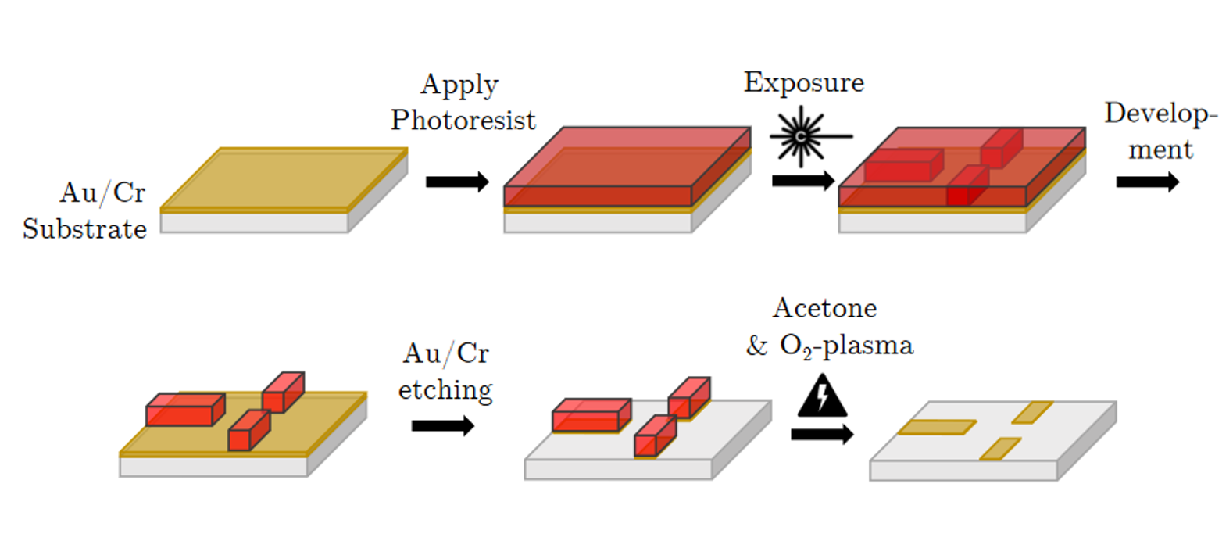
\includegraphics[width=10cm]{Images/pdf/Au-patterning.pdf}
	\caption[Visualization of the workflow for Au-contacts patterning.]{Visualization of the workflow for Au-contacts patterning. Image modified based on reference \cite{bongartzOrganicElectrochemicalTransistors2021}.}
	\label{fig:aupat}
\end{figure}

Then p(g3T2-T) films were deposited following the procedure described in the previous section. The patterning of doped-p(g3T2-T) channel follows a similar procedure from references \cite{weissbachPhotopatternableSolidElectrolyte2022}\cite{bongartzOrganicElectrochemicalTransistors2021}, where PEDOT:PSS is being used, with some modifications in the exposure and developing times. The patterning of undoped-p(g3T2-T) samples, on the other hand, follows a different protocol, the addition of a sacrificial layer is needed to ensure cross-linking. Both processes are described in the following:

\paragraph{Patterning undoped-p(g3T2-T).}Patterning of the p(g3T2-T) was achieved with photolithography, as shown in Figure \ref{fig:undopedpat}. First, a fluoropolymer Sacrificial Layer 1 (SL1) was spin coated at 6000 RPM for 60 s, followed by a baking step for 180 s at $113^{\circ}$C. Before the deposition of photoresist, a O$_{2}$ plasma cleaning step was applied for 60 s to promote adhesion. Then, NLOF 2020 photoresist was spin coated at 3000 RPM for 60 s and baked for another 60 s at $113^{\circ}$C. Exposure of negative resist was performed for 12 s by shadowing all areas except the ones of interest. After post-baking for 60 s at $113^{\circ}$C, NLOF was developed by rinsing the sample in AZ MIF 726 for 20 s and wash off in DI water (carried out extra times if necessary). Next, SL1 was developed using HF 7300 developer for 45 s and spin rinsed at 3000 RPM (carried out extra times if necessary). Excess of p(g3T2-T) was removed by O$_{2}$-plasma etching for 180 s. The sample was placed in Orthogonal Stripper 900 overnight at room temperature, to complete the removal. Finally, ultrasonication in acetone was added for 15 min the next day. 

\begin{figure}[ht]
	\centering
	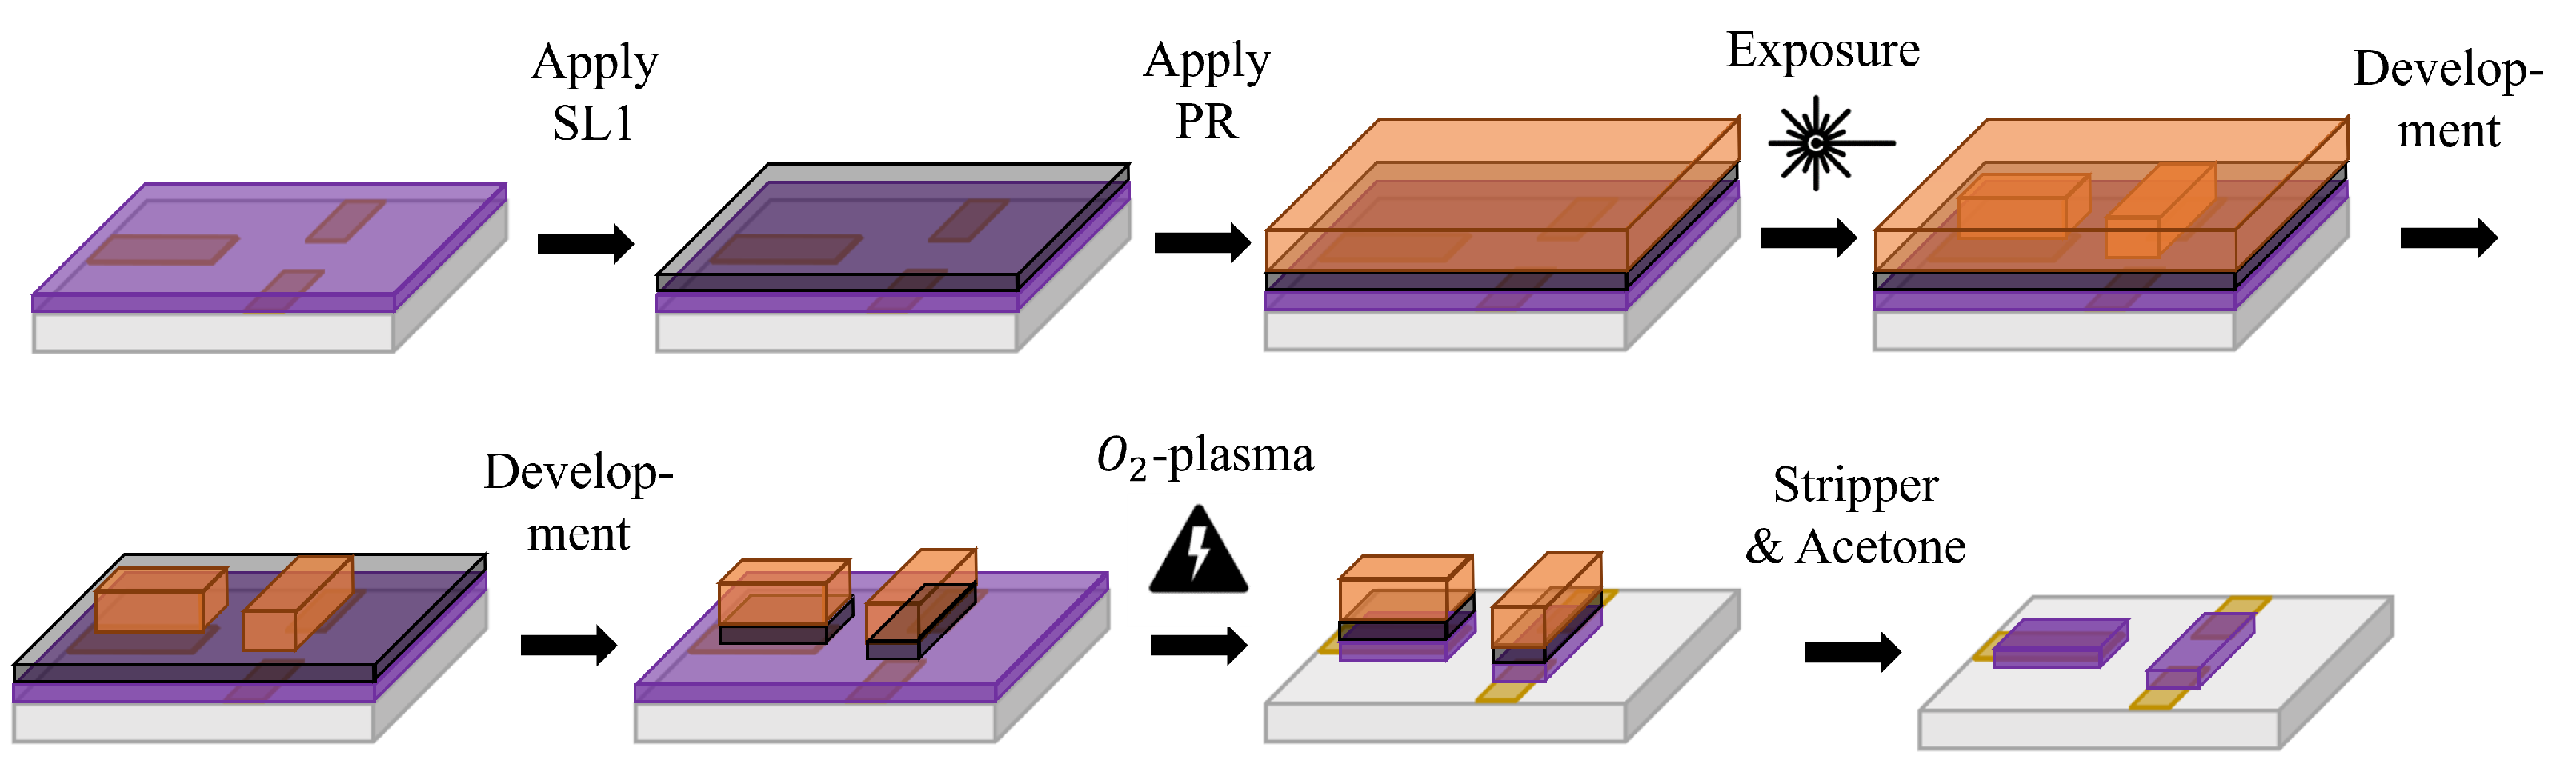
\includegraphics[width=12cm]{Images/pdf/undoped-patterning.pdf}
	\caption{Visualization of the workflow for patterning undoped p(g3T2-T).}
	\label{fig:undopedpat}
\end{figure}

\paragraph{Patterning doped-p(g3T2-T).}Patterning of the doped-p(g3T2-T) was achieved with photolithography, as shown in Figure \ref{fig:dopedpat}. First, the orthogonal photoresist OSCoR 4020 was spin coated at 3000 RPM for 60 s and baked for another 60 s at $103^{\circ}$C. Exposure of negative resist was performed for 20 s with shadowing all areas except the ones of interest, one extra cycle was added if using higher dopant concentration (10 mg/mL). After post-baking for 60 s at $103^{\circ}$C, OSCoR was developed using Orthogonal Developer 103a for 45 s and spin rinsed at 3000 RPM for 60 s (carried out extra times if necessary). Excess of doped-p(g3T2-T) was removed by O$_{2}$-plasma etching for 180 s. The sample was placed in Orthogonal Stripper 900 overnight at room temperature.

\begin{figure}[ht]
	\centering
	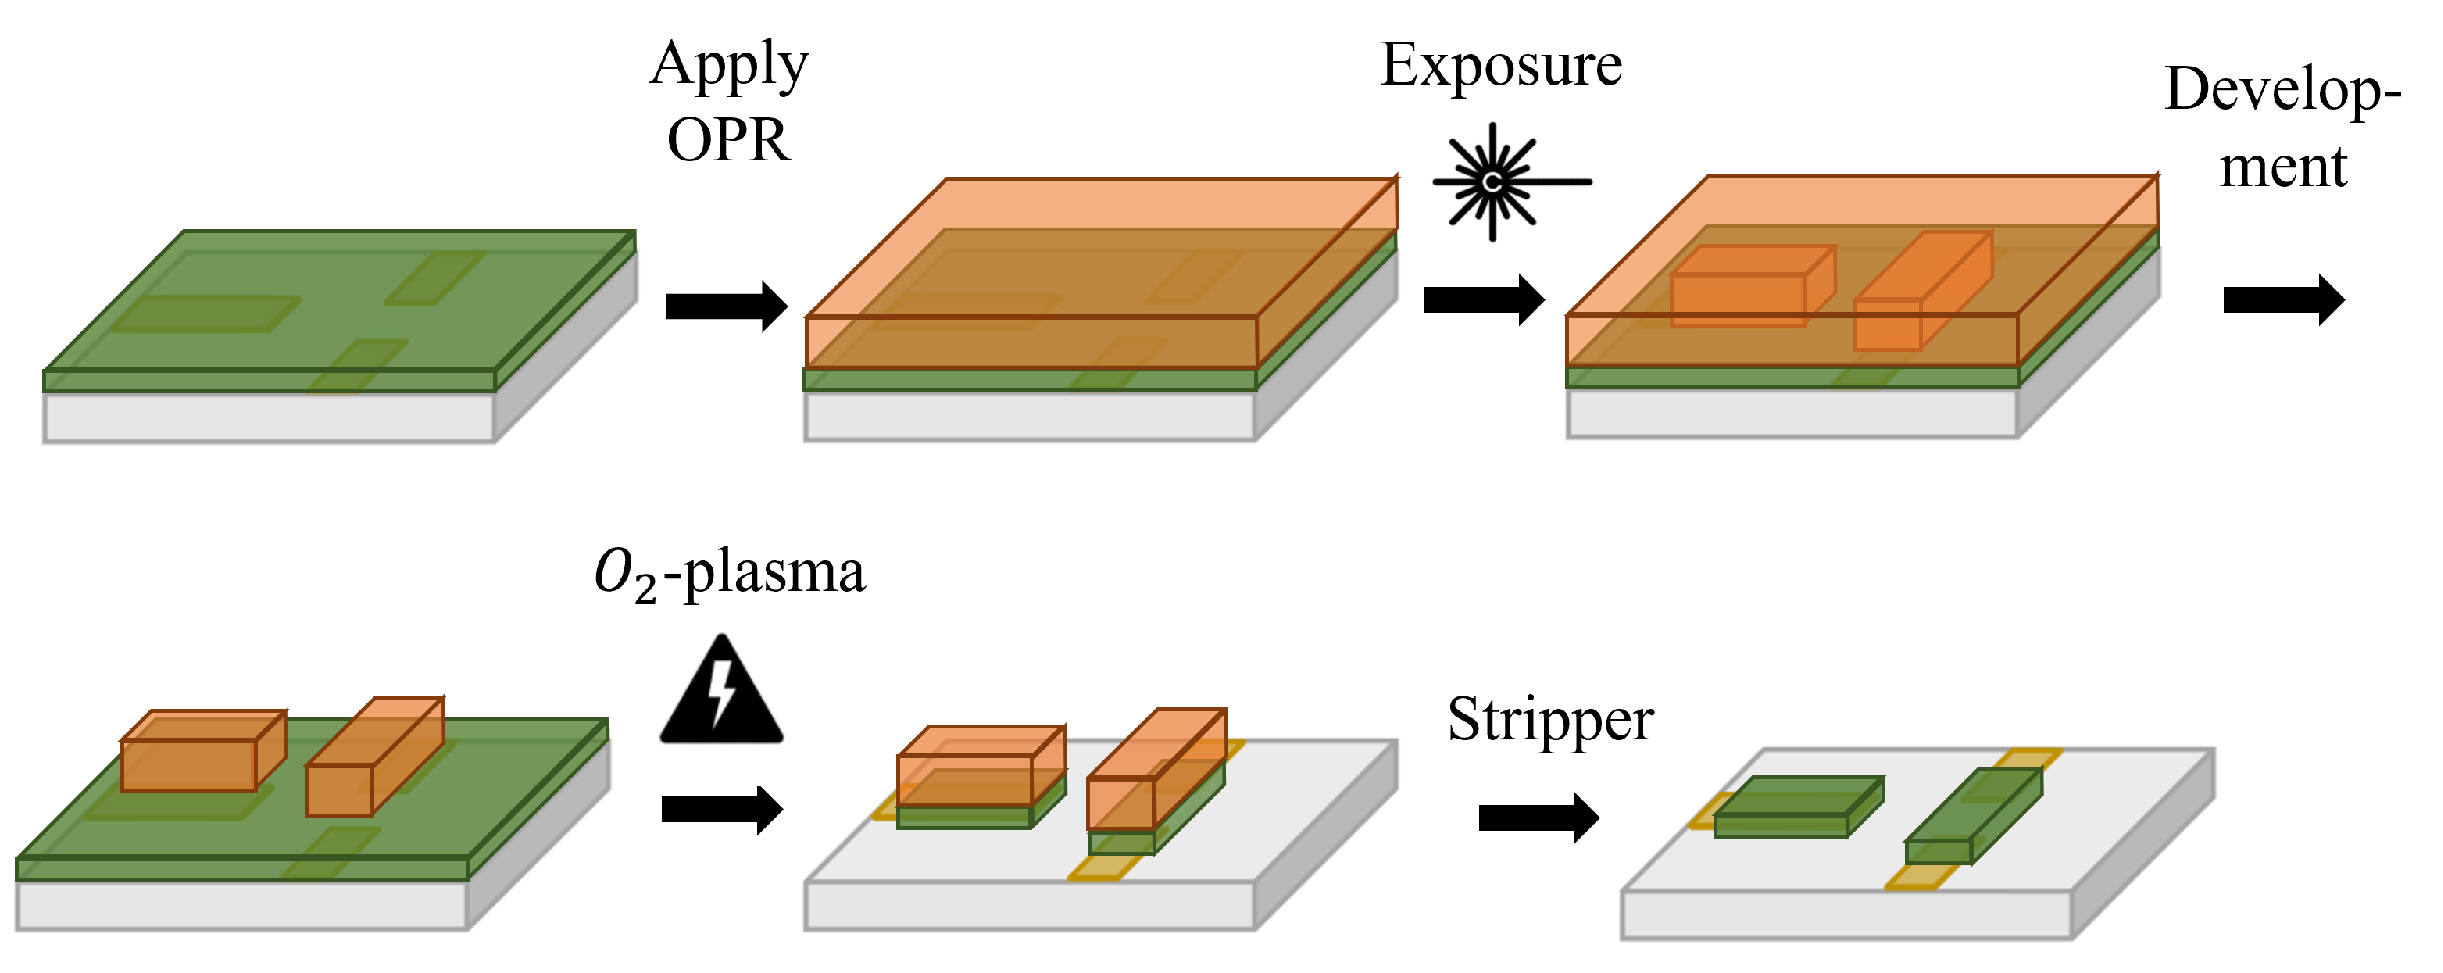
\includegraphics[width=9cm]{Images/pdf/doped-patterning.pdf}
	\caption{Visualization of the workflow for patterning doped p(g3T2-T).}
	\label{fig:dopedpat}
\end{figure}

\paragraph{OECT with undoped- and doped-p(g3T2-T) channel.} A solid-state electrolyte precursor was prepared, as describe in Table \ref{tab:sse}, and 20$\mu$L were dropcasted to the patterned samples (undoped and doped) covering all 14 devices in the sample. Finally, a Ag/AgCl pellet was installed and used as gate (Figure \ref{fig:biosetup}). Transfer characteristics were measured under ambient conditions with different source-drain voltages (V$_{DS}$= -0.1, -0.2, -0.5V).

\begin{table}[h]
	\centering
	\caption{Composition of the solid-state electrolyte \cite{weissbachPhotopatternableSolidElectrolyte2022}.}
	\begin{tabular}{r c l} \hline
		Component   & Amount & Function \\ \hline
		H$_{2}$O	& 1.0 mL & dilution \\ 
		$[$EMIM$][$EtSO$_{4}]$   & 1.5 mL & ionic liquid \\ 
		MBBAm   & 20 mg & crosslinker \\ 
		NIPAm   & 750 mg & monomer \\ 
		HHPAA   & 200 mg & photoinitiator \\
		EG	& 1.5 mL	& increase viscosity, ensures good print \\ 
		Triton & 1 drop & surfactant, ensures good print \\  \hline
	\end{tabular}
	\label{tab:sse}
\end{table}

\begin{figure}[!ht]
	\centering
	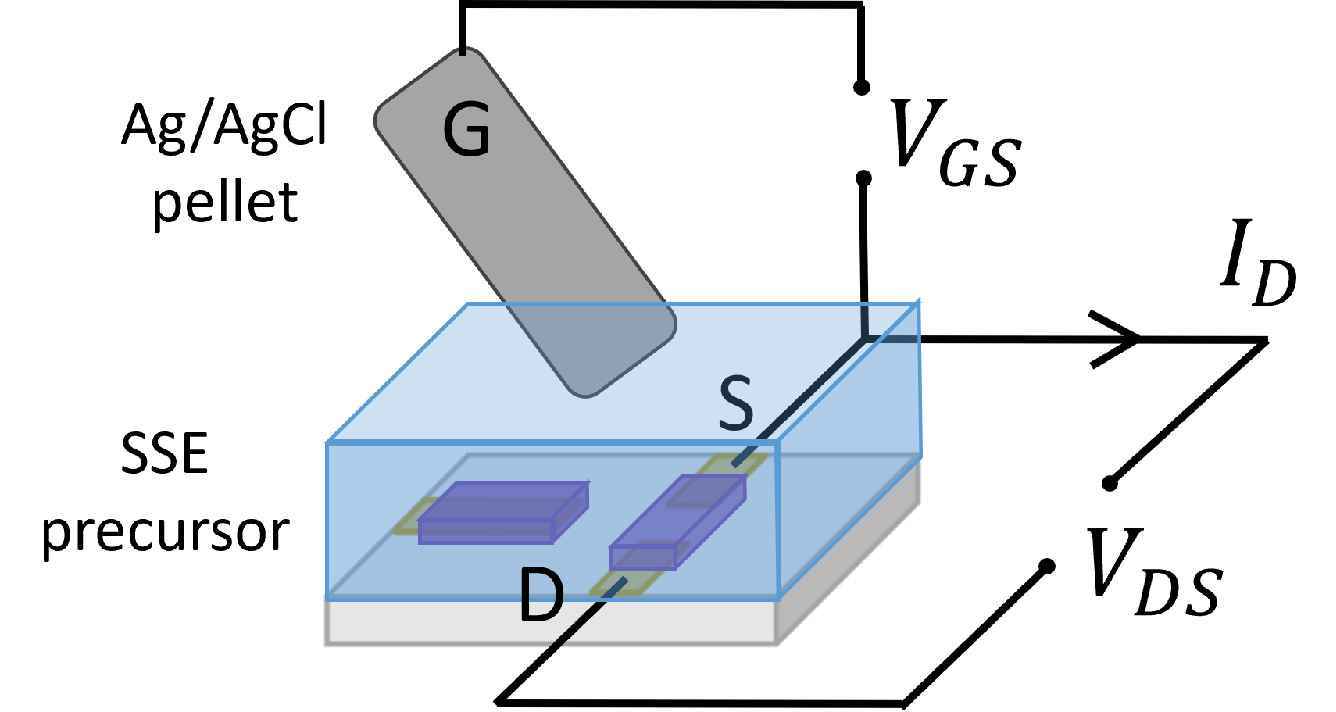
\includegraphics[width=7cm]{Images/pdf/bioprobe_setup.pdf}
	\caption{Experimental setup to measure threshold voltage shift under ambient conditions.}
	\label{fig:biosetup}
\end{figure}

%\newpage
\subsubsection{Stability on Air of p(g3T2-T)}
In this subsection, the stability of undoped and doped samples of p(g3T2-T) (doped with F$_{6}$TCNNQ, following same procedure described in subsection \ref{subsec:films}) in N$_{2}$ and ambient conditions were tested at different stages of the photolithography process by measuring the channel conductivity under a fixed biased drain-source voltage. %, upon spin-coating, patterning, i) upon dropcast of solid-state electrolyte precursor, and after exposure, ii) after photopatterned solid-state electrolyte, and finally

\paragraph{Channel conductivity measurements.}Undoped-p(g3T2-T) sample was measured in N$_{2}$ then ambient conditions immediately after spin-coating onto substrate with patterned gold contacts. Then, sample was measured after patterning process (as described in previous section). Finally, upon drop-casting solid-state electrolyte precursor. The doped-p(g3T2-T) channel was measured after patterning and upon dropcasting solid-state electrolyte precursor.

\subsubsection{Reverse Oxidation of Undoped-p(g3T2-T)}

\paragraph{By electrochemical dedoping.}Undoped-p(g3T2-T) samples onto patterned-gold-contacts substrates were prepared. The solid-state-electrolyte precursor was dropcast onto the 14 devices, one device source-drain was negatively-biased and applied a positive gate voltage. Channel conductivity was monitored. Finally, other devices on the sample were measured to detect any effect of the process.

\paragraph{By heating.}An undoped-p(g3T2-T) solid-OECT, whose fabrication will be described in the following subsection (\ref{subsec:solidOECT}), was exposed to ambient conditions, devices were clearly oxidized. The sample was placed on a hot plate at 120$^{\circ}$C, brought back to glovebox, and measured the following day.  %\cite{weissbachPhotopatternableSolidElectrolyte2022}.
%% alcohol rinse
\subsubsection{Solid-OECTs using Undoped-p(g3T2-T)} \label{subsec:solidOECT}
After following the patterning steps for undoped-(pg3T2-T) from Subsection \ref{subsec:photo}. Three different methods of applying the solid-state electrolyte precursor were tested. Then, transfer characteristics at V$_{DS}$=-0.1V at a scanning rate of 0.083 V/s were measured. Cyclic voltammetry and electrochemical impedance spectroscopy was performed by short-circuiting source and drain to probe between channel and gate, parameters were fixed as described in Section \ref{param}, measurements were taken one day after the fabrication.

\paragraph{OECT with dropcasted Solid-State Electrolyte.}Solid-state electrolyte precursor was dropcasted and then exposed for 2 cycles of 60 s in mask aligner, as shown in Figure \ref{fig:undopedsse}A. 

\paragraph{OECT with photopatternable Solid-State Electrolyte.}First, the application of an adhesion promoter was used, composed by reactants from Table \ref{tab:adprom}, the sample was covered in Petri dish at 50$^{\circ}$C, then rinse very thoroughly with ethanol and dried for at least 10 min at 100$^{\circ}$C on hot plate. Composition and application steps of adhesion promoter was previosly defined by Biosens group members at IAPP. Solid-state-electrolyte precursor was dropcasted, then a Teflon foil was placed on top to avoid contact with mask that will shadow all areas except the ones of interest in the negative resist, exposed for 2 cycles of 60 s in mask aligner, and blown off with a N$_{2}$ gun, as shown in Figure \ref{fig:undopedsse}B,  following references \cite{weissbachPhotopatternableSolidElectrolyte2022}\cite{bongartzOrganicElectrochemicalTransistors2021}.

\begin{table}[h]
	\centering
	\caption{Composition of adhesion promoter.}
	\begin{tabular}{r r} \hline
		Component   & Amount \\ \hline
		SilaneA174	& 30 $\mu$L \\ 
		Etanol   & 3mL \\ 
		Acetic acid   & 60 $\mu$L \\ \hline
	\end{tabular}
	\label{tab:adprom}
\end{table}

\paragraph{OECT with inkjet-printed Solid-State Electrolyte.}First, the application of an adhesion promoter as described previosly. Then, the solid-state-electrolyte precursor was ink-jet printed and expose for 2 cycles of 60 s in mask aligner, parameters and procedure for ink-jet printing was previosly established by members of BioSens group at IAPP, as shown in Figure \ref{fig:undopedsse}C. 

\begin{figure}[!ht]
	\centering
	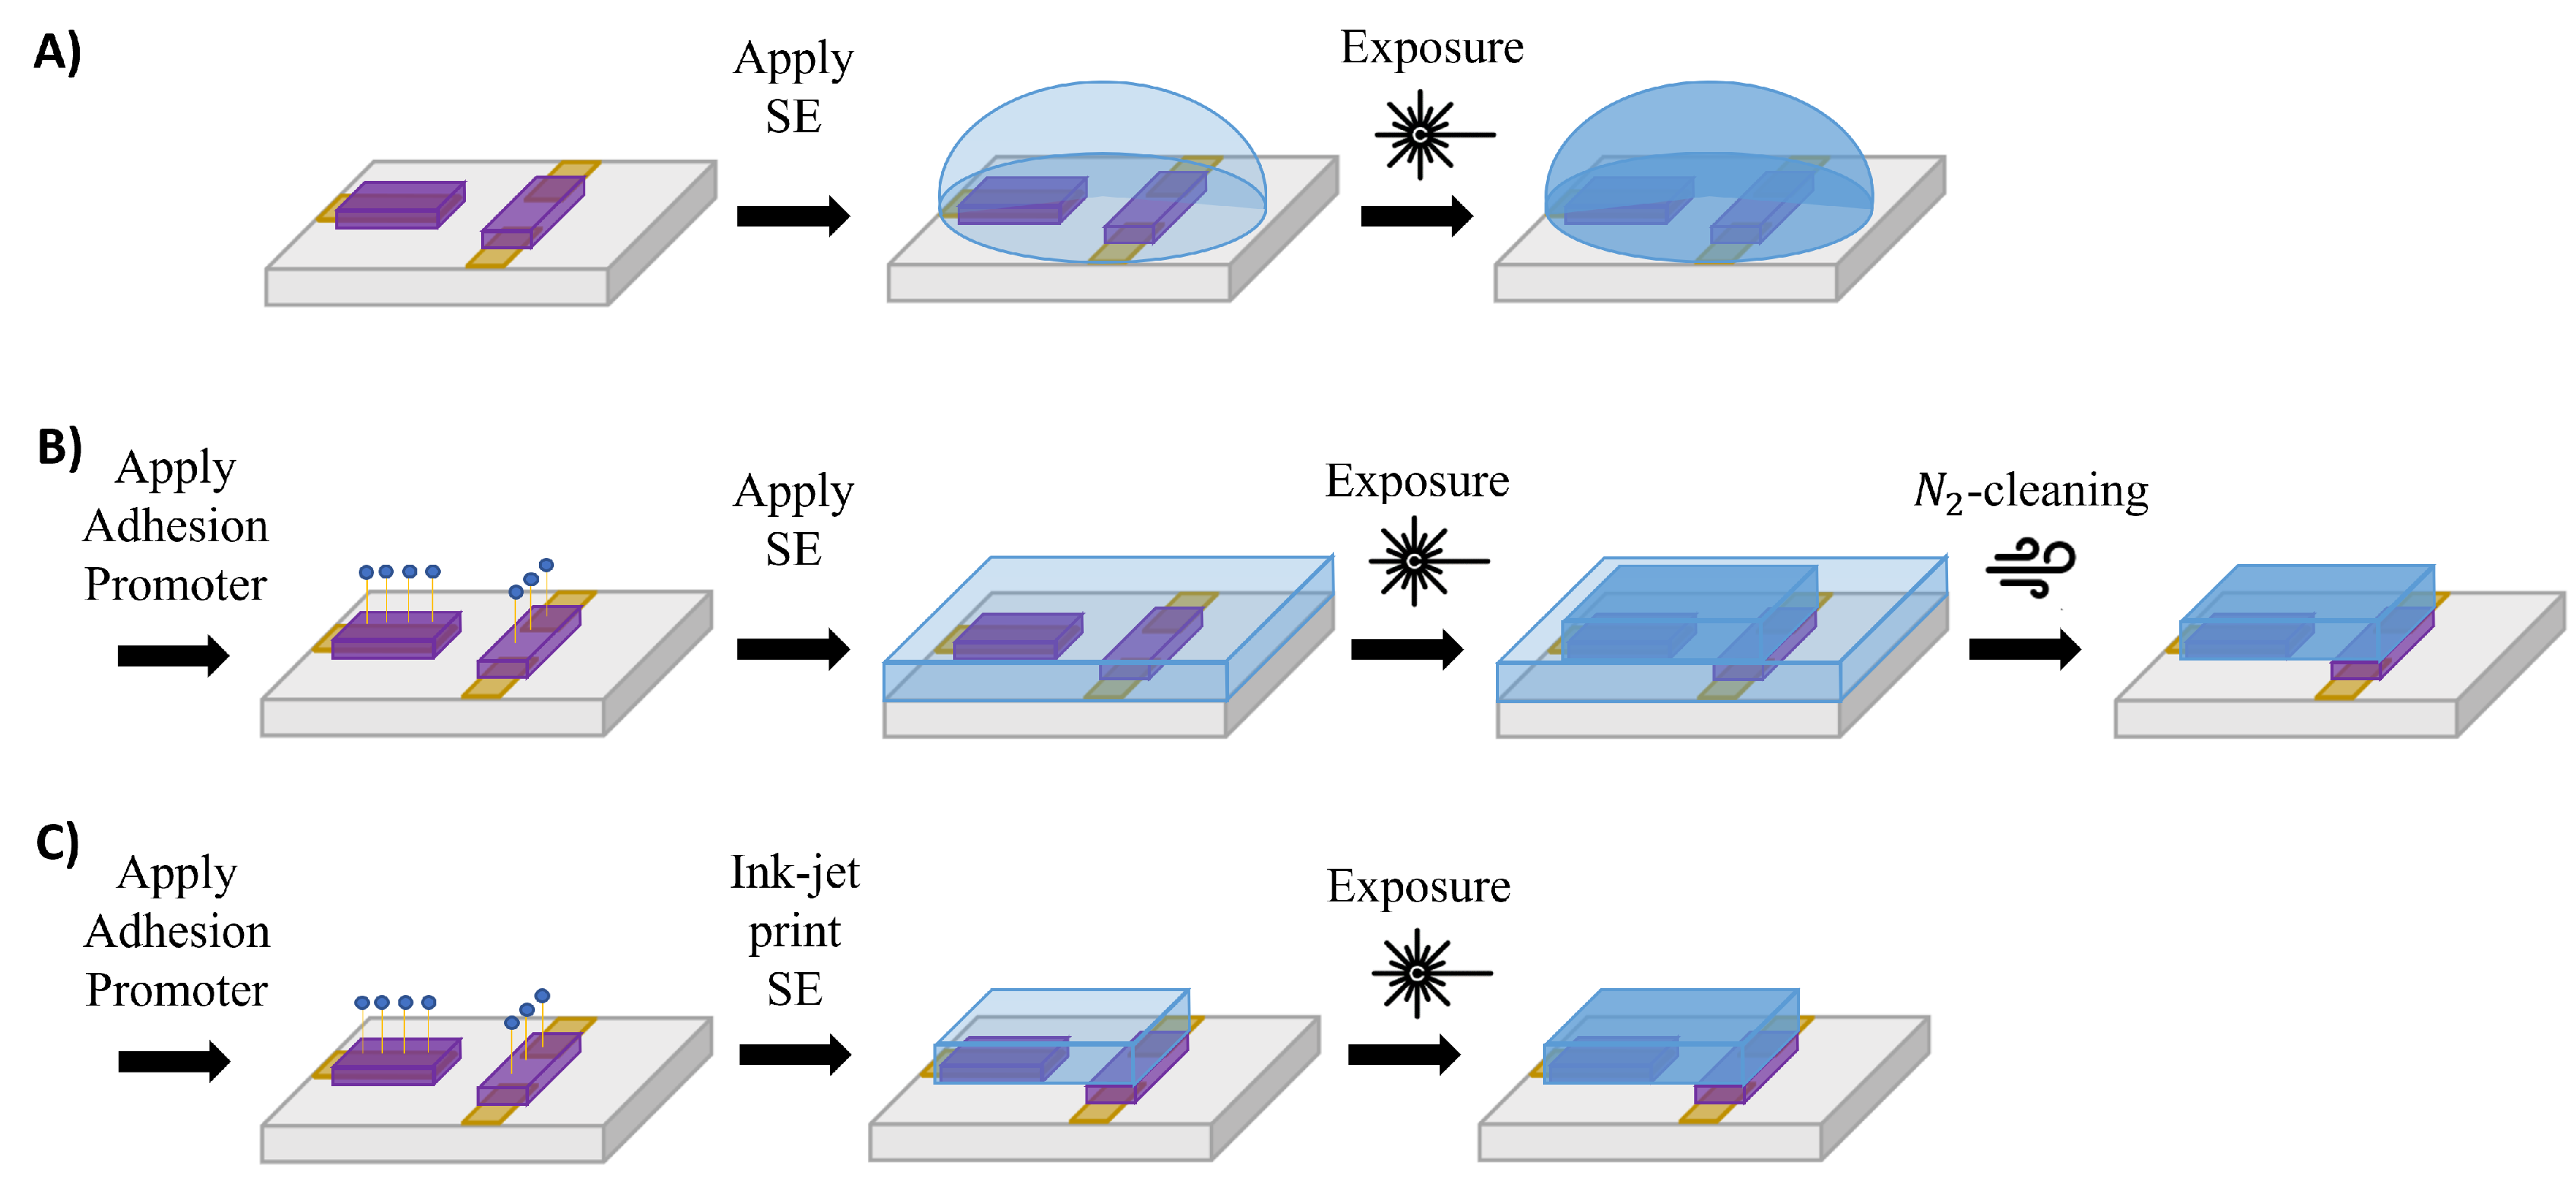
\includegraphics[width=\textwidth]{Images/pdf/undoped-sse.pdf}
	\caption[Solid-OECT fabrication with undoped p(g3T2-T)]{Visualization of the workflow for solid-OECT fabrication with undoped p(g3T2-T) by A) dropcasting SSE, B) photopatterning SSE, C) ink-jet printing SSE.}
	\label{fig:undopedsse}
\end{figure}

\subsubsection{Solid-OECTs using Doped-p(g3T2-T)}

\paragraph{OECT with inkjet-printed Solid-State Electrolyte.}After the deposition of films and dopant (F$_{6}$TCNNQ), films were stored in glovebox over the weekend to let dopants soak and dry. Then, the patterning steps for doped-(pg3T2-T) from Subsection \ref{subsec:photo} were followed with no extra cycles in exposure times. Solid-state-electrolyte precursor was ink-jet printed as described in the previous Subsection. Then, transfer characteristics at V$_{DS}$=-0.1V at a scanning rate of 0.083 V/s were measured. Cyclic voltammetry and electrochemical impedance spectroscopy were performed by short-circuiting source and drain to probe between channel and gate, parameters were fixed as described in section \ref{param}, measurements were taken one day after the fabrication.

\begin{figure}[!ht]
	\centering
	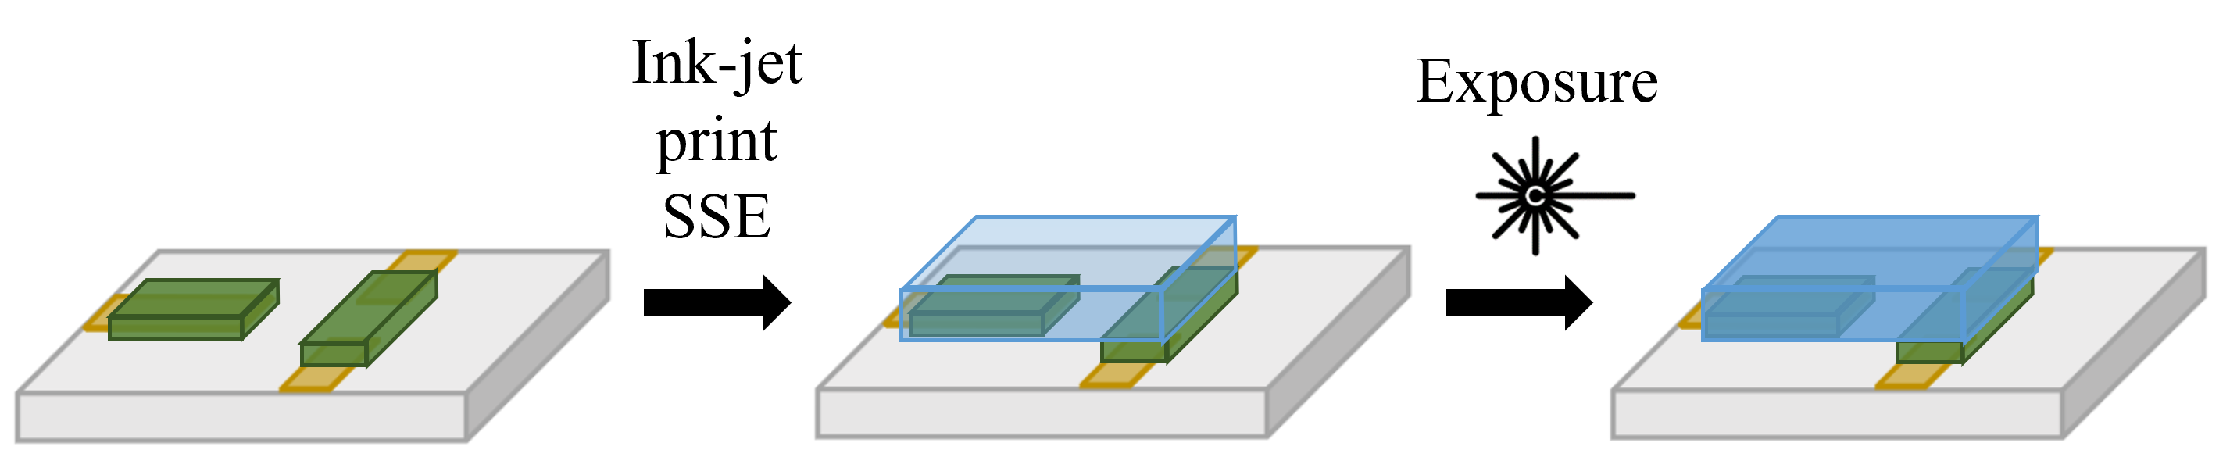
\includegraphics[width=10cm]{Images/pdf/doped-sse.pdf}
	\caption[Solid-OECT fabrication with doped p(g3T2-T)]{Visualization of the workflow for solid-OECT fabrication with doped p(g3T2-T) by ink-jet printing SSE.}
	\label{fig:dopedsse}
\end{figure}

%%% Local Variables: 
%%% mode: latex
%%% TeX-master: "thesis"
%%% End: 
